\documentclass[twocolumn,superscriptaddress,aps]{revtex4-1}

\usepackage[utf8]{inputenc}

\usepackage{amsfonts}
\usepackage{amssymb}
\usepackage{amsmath}
\usepackage{amsthm}

\usepackage{bm}
\usepackage{cancel}
\usepackage{bbold}
\usepackage{bm}
\usepackage{slashed}
\usepackage{graphicx}
\usepackage{color}
\usepackage{hyperref}
\usepackage{algorithm}
\usepackage{algpseudocode}
\usepackage{tikz}

\newcommand{\glnote}[1]{\textcolor{red}{[GL: #1]}}
\newcommand{\kcnote}[1]{\textcolor{red}{[KC: #1]}}

\newcommand{\qxpsi}{q(\mathbf{x}|\bfpsi)}
\newcommand{\bftheta}{{\bm \theta}}
\newcommand{\bfpsi}{{\bm \psi}}
\newcommand{\bfphi}{{\bm \phi}}
\newcommand{\bflambda}{{\bm \lambda}}
\newcommand{\bfx}{\mathbf{x}}
\newcommand{\bfz}{\mathbf{z}}

\theoremstyle{plain}
\newtheorem{theorem}{Theorem}
\newtheorem{proposition}[theorem]{Proposition}

\begin{document}


% ==============================================================================

\title{\Large{Adversarial Variational Optimization of Non-Differentiable Simulators}}
\vspace{1cm}
\author{\small{\bf Gilles Louppe}\thanks{\texttt{g.louppe@nyu.edu}}}
\affiliation{New York University}
\author{\small{\bf Kyle Cranmer}\thanks{\texttt{kyle.cranmer@nyu.edu}}}
\affiliation{New York University}

\begin{abstract}
Complex computer simulators are increasingly used across fields of science as
generative models tying parameters of an underlying theory to
experimental observations. Inference in this setup is often
difficult, as simulators rarely admit a tractable density or likelihood
function. We introduce Adversarial Variational Optimization (AVO), a likelihood-free
inference algorithm for fitting a non-differentiable generative model or to perform empirical Bayes through variational inference.
We adapt the training procedure of generative
adversarial networks by replacing the differentiable generative network with a
domain-specific simulator. We solve the resulting non-differentiable
minimax problem by minimizing variational upper bounds of the two adversarial objectives.
Effectively, the procedure results in learning an arbitrarily tight
proposal distribution over simulator parameters, such that the corresponding
marginal distribution of the generated data matches the observations.
We present results of the method with simulators producing both discrete and continuous data.

\end{abstract}

\maketitle

% ==============================================================================

\section{Introduction}

%Computer simulators are used to describe complex data generation processes in a diverse set of fields of science including particle physics, climatology, epidemiology,  and population
%genetics,

In many fields of science such as particle physics, epidemiology,  and population
genetics, computer simulators are used to describe complex data generation processes. These simulators relate
observations $\bfx$ to the parameters $\bftheta$ of an underlying theory or mechanistic model.
In most cases, these simulators are specified as procedural implementations of forward, stochastic processes involving latent variables $\bfz$.
% and may generate either discrete or continuous data.
Rarely do these simulators admit a tractable density (or likelihood) $p(\bfx |
\bftheta)$. The prevalence and significance of this problem has motivated an
active research effort in so-called \textit{likelihood-free inference}
algorithms such as Approximate Bayesian Computation
(ABC)~\cite{beaumont2002approximate, marjoram2003markov, sisson2007sequential,
sisson2011likelihood, marin2012approximate, cranmer2015approximating}.  Often
the simulation code involves control-flow that implies the dependence of $\bfx$
on $\bfz$ is non-differentiable, making inference even more difficult and
precludes approaches such as Ref.~\citep{2016arXiv160507826G}.

%\kcnote{HMC https://arxiv.org/pdf/1503.01916.pdf}

%\kcnote{add ABC refs mentioned in tex}
%(Beaumont et al., 2002; Marjoram et al., 2003; Sisson et al., 2007; Sisson \& Fan, 2010; Marin et al., 2012; Fan et al., 2013) }

%Often the simulation code involves control-flow that leads to models such that even $p(\bfx | \bftheta)$ is non-differentiable with respect to $\bftheta$, making inference even more difficult and precluding approaches such as Ref.~\citep{2016arXiv160507826G}.

In parallel, with the introduction of variational
auto-encoders~\citep{DBLP:journals/corr/KingmaW13} and generative adversarial
networks~\cite{goodfellow2014generative}, there has been a vibrant research
program around implicit generative models based on neural
networks~\citep{2016arXiv161003483M}.  While these implicit generative networks
also do not admit a tractable density, they are differentiable.


%%In contrast, scientific simulators involve control-flow that leads to models such that $p(\bfx, \bfz | \bftheta)$ is non-differentiable with respect to $\bftheta$, making inference even more difficult and precluding approaches such as Ref.~\citep{2016arXiv160507826G}.
%Scientific simulators can be thought of as highly regularized generative models as they typically have relatively few parameters  endowed with some level of interpretation. In contrast, generative models based on neural networks are highly parametrized and the model parameters have no obvious interpretation. In this setting, inference on the model parameters $\bftheta$ is often of more interest than the latent variables $\bfz$.



%While generative models based on neural networks are highly parametrized and the model parameters have no obvious interpretation, scientific simulators typically have relatively few parameters that endowed with some level of interpretation. Thus simulators can be thought of as highly regularized, non-differentiable generative models. In this setting, inference on the model parameters $\bftheta$ is often of more interest than the latents $\bfz$.

%Generative models based on neural networks are differentiable with respect to their high dimensional model parameters $\bftheta$, which  with no particular , differentiable with respect to $\bfz$ and $\bftheta$, and the distribution of the latent $\bfz$
%
%In the context of variational inference, one assumes the the likelihood $p(\bfx | \bftheta)$ is available and posterior $p(\bftheta | \bfx)$ is tractable up to a constant (ie. ($p(\bfx, \bfz | \bftheta)$ is tractable). Moreover, one is typically interested in estimating the posterior distribution of the latent variables instead of the parameters of the simulator $\bftheta$.


%In the context of variational inference, these technihave also been used as the recognition model ~\citep{2015arXiv150505770J, DBLP:journals/corr/KingmaSW16, DBLP:conf/icml/RezendeMW14}; however, in those cases the likelihood $p(\bfx | \bftheta)$ is available and posterior $p(\bftheta | \bfx)$ is tractable up to a constant.

%Because it is usually computationally intractable, most simulators
%
%implicit generative models~\citep{2016arXiv161003483M}
%
%In most
%cases, these implicit generative models~\citep{2016arXiv161003483M} are
%specified as procedural implementations of forward stochastic processes that
%generates discrete or continuous data, and rarely do these simulators admit a tractable density. Because it is usually computationally intractable, most simulators
%do not provide a way to directly evaluate the likelihood function for a
%given observation, thereby making inference difficult.
%In addition, most scientific simulators are written using opaque low-level programming
%languages, hence raising the bar for likelihood-free inference
%algorithms relying e.g. on the simulator being a function with computable derivatives~\citep{2016arXiv160507826G}
%or being a controllable probabilistic program~\citep{2016arXiv161009900L}.

Generative models based on neural networks are highly parametrized and the model
parameters have no obvious interpretation. In contrast, scientific simulators
can be thought of as highly regularized generative models as they typically have
relatively few parameters and they are endowed with some level of
interpretation. In this setting, inference on the model parameters $\bftheta$ is
often of more interest than the latent variables $\bfz$.

In this note, we develop an unsupervised learning algorithm for the point
estimation of the parameters $\bftheta$ of a non-differentiable, implicit
generative model. We adapt the adversarial
training procedure of generative adversarial
networks~\cite{goodfellow2014generative} by replacing the implicit generative
network with a domain-based scientific simulator, and solve the resulting
non-differentiable minimax problem by minimizing variational upper
bounds~\citep{2011arXiv1106.4487W,2012arXiv1212.4507S} of the adversarial
objectives. The procedure results in learning an arbitrarily tight
proposal distribution over simulator parameters, such that the corresponding
marginal distribution of the generated data matches the observations.


%In this note, we develop a likelihood-free inference algorithm for the point
%estimation of the parameters $\bftheta$ of a non-differentiable, implicit
%generative model. We adapt the adversarial
%training procedure of generative adversarial
%networks~\cite{goodfellow2014generative} by replacing the implicit generative
%network with a domain-based scientific simulator, and solve the resulting
%non-differentiable minimax problem by minimizing variational upper
%bounds~\citep{2011arXiv1106.4487W,2012arXiv1212.4507S} of the adversarial
%objectives. The procedure results in learning a proposal distribution over
%simulator parameters, hence producing an arbitrarily tight family of models whose
%marginal distribution of generated data matches the observed data.


% ==============================================================================

\section{Problem statement}
\label{sec:problem}

We consider a family of parametrized densities $p(\mathbf{x}|\bftheta)$
defined implicitly through the simulation of a stochastic generative process,
where $\mathbf{x} \in \mathbb{R}^d$ is the data and $\bftheta$ are the
parameters of interest. The simulation may involve some complicated latent
process
%, such that
%\begin{equation}\label{eqn:p_x}
%    p(\mathbf{x}|\bftheta) = \int p(\mathbf{x}|\bfz,\bftheta) p(\bfz|\bftheta) d\bfz
%\end{equation}
%\begin{equation}\label{eqn:p_x_sim}
%    p(\mathbf{x}|\bftheta) = \frac{\partial}{\partial x_1} \dots \frac{\partial}{\partial x_d} \int_{\{\bfz:g(\bfz;\bftheta) \leq \mathbf{x}\}} p(\bfz|\bftheta) \mu(d\bfz),
%\end{equation}
where $\bfz \in {\cal Z}$ is a latent variable providing an external
source of randomness.
Unlike implicit generative models defined by neural networks, we do not assume
$\bfz$ to be a fixed-size vector with a simple density. Instead, the
dimension of $\bfz$ and the nature of its components (uniform, normal,
discrete, continuous, etc.) are inherited from the control flow of the
simulation code and may depend on $\bftheta$ in some intricate way. Moreover,
the dimension of $\bfz$ may be much larger than the dimension of
$\bfx$. Thus we do not attempt to learn a recognition model $q(\bfz | \bfx)$.

%Unlike implicit generative models defined by neural networks, we do not assume $\bfz$ to
%be a fixed-size vector (e.g., it can be a sequence of variable length) and its
%distribution $p(\bfz|\bftheta)$ may itself depend on $\bftheta$ in some intricate way
%inherited from the control flow of the simulation code.

We assume that the stochastic generative process that defines $p(\mathbf{x}|\bftheta)$ is
specified through a non-differentiable deterministic function $g(\cdot; \bftheta) : {\cal Z} \to
\mathbb{R}^d$. Operationally, %That is, we consider
\begin{equation}\label{eqn:p_theta}
    \mathbf{x} \sim p(\mathbf{x}|\bftheta) \equiv \bfz \sim p(\bfz|\bftheta), \mathbf{x} = g(\bfz; \bftheta)
\end{equation}
such that the density $p(\mathbf{x}|\bftheta)$ can be
written as
%considered as a non-differentiable reparameterization of the random variable $\bfz$
%\begin{equation}\label{eqn:p_x_sim}
%    p(\mathbf{x}|\bftheta) = \frac{\partial}{\partial x_1} \dots \frac{\partial}{\partial x_d} \int_{\{\bfz:g_i(\bfz;\bftheta) \leq x_i\}} p(\bfz|\bftheta) \mu(d\bfz),
%\end{equation}
\begin{equation}\label{eqn:p_x_sim}
    p(\mathbf{x}|\bftheta) = \int_{\{\bfz:g(\bfz;\bftheta) = \bfx \}} p(\bfz|\bftheta) \mu(d\bfz),
\end{equation}
where $\mu$ is a probability measure.
%Importantly, the simulator $g$ is assumed to be a non-invertible function, that can only be
%used to generate data in forward mode. For this reason, evaluating the integral
%in Eqn.~\ref{eqn:p_x_sim} is intractable. As commonly found
%in science, we finally assume the lack of access to or existence of derivatives of $g$ with respect to $\bftheta$,
%e.g. as when $g$ is specified as a computer program.

Given some observed data $\{ \mathbf{x}_i | i=1, \dots, N \}$ drawn from the
(unknown) true distribution $p_r(\mathbf{x})$, our goal is to estimate the parameters
$\bftheta^*$ that minimize the divergence between $p_r(\mathbf{x})$ and
the implicit model $p(\mathbf{x}|\bftheta)$. That is,
\begin{equation}
    \bftheta^* = \arg \min_{\bftheta \in \bftheta} \rho(p_r(\mathbf{x}), p(\mathbf{x}|\bftheta)),
\end{equation}
where $\rho$ is some distance or divergence.
%~\citep{bernton2017inference}.
%For many choices of divergence $\rho$, this is asymptotically equivalent to a maximum likelihood estimate if $ \rho(p_r(\mathbf{x}), p(\mathbf{x}|\bftheta^*)) \to 0$.


%By plugging Wp in place of D in Eqs. (1) and (2), we obtain the minimum Wasserstein estimator (MWE) and minimum expected Wasserstein estimator (MEWE) of order p, denoted ??n and ??n,m respectively. Some properties of the MWE have been studied in Bassetti et al. (2006), for well-specified models and i.i.d. data; we propose new results in Section 4. Intuitively, under some conditions we can expect ??n to converge to ??, in the sense that Wp(??n,??) ? 0. Consequently, the minimum of ?  ? Wp(??n,??) might converge to the minimum of ?  ? Wp(??,??), denoted by ??, assuming its existence and unicity. In the well-specified case, ?? coincides with the data-generating parameter. In the misspecified case, ?? is typically different from the limit of the maximum likelihood estimator (MLE), which is the minimizer of KL(??|??).

% ==============================================================================

\section{Background}

\subsection{Generative adversarial networks}
\label{sec:gans}

Generative adversarial networks (GANs) were first proposed by
\cite{goodfellow2014generative} as a way to build an implicit generative model
capable of producing samples from random noise $\bfz$. More specifically,
a generative model $g(\cdot; \bftheta)$ is pit against an adversarial
classifier $d(\cdot; \bfphi):\mathbb{R}^d \to [0,1]$ with parameters $\bfphi$ and whose antagonistic objective is to recognize real data $\mathbf{x}$
from generated data $\tilde{\mathbf{x}} = g(\bfz; \bftheta)$. Both models $g$ and $d$
are trained simultaneously, in such a way that $g$ learns to fool
its adversary $d$ (which happens when $g$ produces samples comparable to the
observed data), while $d$ continuously adapts to changes in $g$. When $d$ is
trained to optimality before each parameter update of the generator, it can
be shown that the original adversarial learning procedure~\cite{goodfellow2014generative} amounts to minimizing
the Jensen-Shannon divergence $\text{JSD}(p_r(\mathbf{x}) \parallel p(\mathbf{x}|\bftheta))$ between $p_r(\mathbf{x})$ and $p(\mathbf{x}|\bftheta)$.

As thoroughly explored in \citep{2017arXiv170104862A}, GANs remain remarkably
difficult to train because of vanishing gradients as $d$ saturates, or because of
unreliable updates when the training procedure is relaxed. As a remedy,
Wasserstein GANs~\citep{2017arXiv170107875A} reformulate the adversarial
setup in order to minimize the Wasserstein-1 distance $W( p_r(\mathbf{x} ), p(\mathbf{x} | \bftheta)  )$
by replacing the adversarial classifier with a 1-Lipschitz adversarial critic
$d(\cdot; \bfphi) : \mathbb{R}^d \to \mathbb{R}$, and where
\begin{align}
& W( p_r(\mathbf{x} ), p(\mathbf{x} | \bftheta)  ) \nonumber \\
&= \sup_{\bfphi}  \mathbb{E}_{\tilde{\mathbf{x}}\sim p(\mathbf{x}|\bftheta)} [d(\tilde{\mathbf{x}}; \bfphi)] - \mathbb{E}_{\mathbf{x} \sim p_r(\mathbf{x})} [d(\mathbf{x}; \bfphi)] \nonumber \\
&\equiv \sup_{\bfphi} \mathcal{L}_W.
\end{align}
Under the WGAN-GP formulation of \cite{2017arXiv170400028G}
for stabilizing the optimization procedure,
training $d$ and $g$ results in alternating gradient updates on $\bfphi$ and $\bftheta$ in order to respectively minimize
\begin{align}
    {\cal L}_d =\,&  \mathcal{L}_W + \lambda \mathbb{E}_{\hat{\mathbf{x}} \sim p({\hat{\mathbf{x}})}} [(|| \nabla_{\hat{\mathbf{x}}} d({\hat{\mathbf{x}}};\bfphi) ||_2 - 1)^2] \\
    {\cal L}_g =\,& - \mathcal{L}_W
\end{align}
%
%\begin{align}
%    {\cal L}_d =\,&  {\cal L}_W + \lambda \mathbb{E}_{\hat{\mathbf{x}} \sim p({\hat{\mathbf{x}})}} [(|| \nabla_{\hat{\mathbf{x}}} d({\hat{\mathbf{x}}};\bfphi) ||_2 - 1)^2] \\
%    {\cal L}_g =\,& - {\cal L}_W
%\end{align}
%\begin{align}
%    {\cal L}_d =\,& \mathbb{E}_{\tilde{\mathbf{x}} \sim p(\mathbf{x}|\bftheta)} [d(\tilde{\mathbf{x}};\bfphi)] - \mathbb{E}_{\mathbf{x} \sim p_r(\mathbf{x})} [d(\mathbf{x};\bfphi)]  \nonumber \\
%                  & + \lambda \mathbb{E}_{\hat{\mathbf{x}} \sim p({\hat{\mathbf{x}})}} [(|| \nabla_{\hat{\mathbf{x}}} d({\hat{\mathbf{x}}};\bfphi) ||_2 - 1)^2] \\
%    {\cal L}_g =\,& -\mathbb{E}_{\tilde{\mathbf{x}} \sim p(\mathbf{x}|\bftheta)} [d(\tilde{\mathbf{x}};\bfphi)]
%\end{align}
where ${\hat{\mathbf{x}}} := \epsilon \mathbf{x} +
(1-\epsilon)\tilde{\mathbf{x}}$, for $\epsilon \sim U[0,1]$, $\mathbf{x} \sim
p_r(\mathbf{x})$ and $\tilde{\mathbf{x}} \sim p(\mathbf{x}|\bftheta)$.


\subsection{Variational optimization}

Variational optimization~\cite{2012arXiv1212.4507S,staines2013optimization} and evolution strategies~\citep{2011arXiv1106.4487W} are general
optimization techniques that can be used to form a differentiable bound
on the optima of a non-differentiable function. Given a function $f$ to minimize,
these techniques are based on the simple fact that
\begin{equation}
    \min_{\bftheta \in {\Theta}} f(\bftheta) \leq \mathbb{E}_{\bftheta \sim q(\bftheta|\bfpsi)} [f(\bftheta)] = U(\bfpsi),
\end{equation}
where $q(\bftheta|\bfpsi)$ is a proposal distribution with parameters $\bfpsi$ over input values $\bftheta$.
That is, the minimum of a set of function values is always less than or equal
to any of their average. Provided that the proposal is flexible enough, the parameters $\bfpsi$
can be updated to place its mass arbitrarily tight around the optimum $\bftheta^* = \min_{\bftheta \in \Theta} f(\bftheta)$.

Under mild restrictions outlined in  \citep{2012arXiv1212.4507S}, the bound
$U(\bfpsi)$ is differentiable with respect to $\bfpsi$, and using the log-likelihood
trick it can be rewritten as:
\begin{align}\label{eqn:approx-grad}
    \nabla_\bfpsi U(\bfpsi) &= \nabla_\bfpsi \mathbb{E}_{\bftheta \sim q(\bftheta|\bfpsi)} [f(\bftheta)] \nonumber \\
    %&= \nabla_\bfpsi \int f(\bftheta)  q(\bftheta|\bfpsi)  d\bftheta \nonumber \\
 %   &= \int f(\bftheta) \nabla_\bfpsi q(\bftheta|\bfpsi)  d\bftheta \nonumber \\
   % &= \int \left[ f(\bftheta) \nabla_\bfpsi \log q(\bftheta|\bfpsi) \right]  q(\bftheta|\bfpsi) d\bftheta \nonumber \\
    &= \mathbb{E}_{\bftheta \sim q(\bftheta|\bfpsi)} [f(\bftheta) \nabla_\bfpsi \log q(\bftheta|\bfpsi)]
\end{align}
Effectively, this means that provided that the score function $\nabla_\bfpsi \log
q(\bftheta|\bfpsi)$ of the proposal is known and that one can evaluate
$f(\mathbf{\bftheta})$ for any $\bftheta$, then one can construct empirical
estimates of Eqn.~\ref{eqn:approx-grad}, which can in turn be used to minimize
$U(\bfpsi)$ with stochastic gradient descent. We will use
Adam~\cite{2014arXiv1412.6980K}, but note the opportunity to incorporate the Natural Evolution Strategy
algorithm~\citep{2011arXiv1106.4487W} and variance reduction techniques~\citep{ranganath2014black}.
%Algorithm~\ref{alg:avo} represents the simplest version of AVO; however, the variance of the noisy estimator of the gradients may be too large to be useful in many problems. Variance reduction techniques such as Rao-Blackwellization and Control Variates can be applied here as they are in black box variational inference~\citep{ranganath2014black}.


% In this simple form, stochastic gradient descent based on
% Eqn~\ref{eqn:approx-grad} is known to suffer from premature convergence and lack
% of scale invariance. To avoid the dependence on the parameterization of the
% proposal distribution, natural gradients~\citep{amari1998natural} can be used
% instead to point towards the steepest descent in the space of realizable
% proposal distributions, rather than in the space of their parameters. Effectively,
% the natural evolution strategy (NES) algorithm~\citep{2011arXiv1106.4487W}
% corrects the gradient of $U$ according to the local curvature of the KL-divergence
% surface of proposal distributions, which results in forming
% \begin{equation}\label{eqn:approx-grad-nat}
%     \tilde{\nabla}_\bfpsi U(\bfpsi) = \mathbf{F}(\bfpsi)^{-1} \nabla_\bfpsi U(\bfpsi),
% \end{equation}
% where $\mathbf{F}(\bfpsi)$ is the Fisher information matrix
% \begin{equation}
%     \mathbf{F}(\bfpsi) = \mathbb{E}_{\bftheta \sim q_\bfphi}[ \nabla_\bfpsi \log q_\bfpsi(\bftheta) \nabla_\bfpsi \log q_\bfpsi(\bftheta)^{\top} ]
% \end{equation}
% and can be estimated from samples, in particular by reusing the derivatives $\nabla_\bfpsi \log q_\bfpsi(\bftheta)$ already
% evaluated to form $\nabla_\bfpsi U(\bfpsi)$.



% ==============================================================================

\section{Adversarial variational optimization}


\begin{figure*}
    \begin{minipage}{\linewidth}
    \begin{algorithm}[H]
    \caption{Adversarial variational optimization (AVO).}

    \begin{flushleft}
        {\it Inputs:} observed data $\{ \mathbf{x}_i \sim p_r(\mathbf{x}) \}_{i=1}^N$, simulator $g$.\\
        {\it Outputs:} proposal distribution $q(\bftheta|\bfpsi)$, such that $\qxpsi \approx p_r(\mathbf{x})$.\\
        {\it Hyper-parameters:} The number $n_{\text{critic}}$ of training iterations of $d$; the size $M$ of a mini-batch; the gradient penalty coefficient $\lambda$; the entropy penalty coefficient $\gamma$.
    \end{flushleft}

    \label{alg:avo}
    \begin{algorithmic}[1]
        \State{$q(\bftheta|\bfpsi) \leftarrow \text{prior on $\bftheta$ (with differentiable and known density)}$}
        \While{$\bfpsi$ has not converged}
            \For{$i=1$ to $n_{\text{critic}}$} \Comment{Update $d$}
                \State{Sample a mini-batch $\{\mathbf{x}_m \sim p_r(\mathbf{x}), \bftheta_m \sim q(\bftheta|\bfpsi), \bfz_m \sim p(\bfz|\bftheta_m), \epsilon_m \sim U[0,1] \}_{m=1}^M$.}
                \For{$m=1$ to $M$}
                    \State{$\tilde{\mathbf{x}}_m \leftarrow g(\bfz_m; \bftheta_m)$}
                    \State{$\hat{\mathbf{x}}_m \leftarrow \epsilon_m \mathbf{x}_m + (1 - \epsilon_m) \tilde{\mathbf{x}}_m$}
                    \State{$U_d^{(m)} \leftarrow d(\tilde{\mathbf{x}}_m; \bfphi) - d(\mathbf{x}_m; \bfphi) + \lambda (|| \nabla_{\hat{\mathbf{x}}_m} d(\hat{\mathbf{x}}_m; \bfphi) ||_2 - 1)^2 $}
                \EndFor
                \State{$\bfphi \leftarrow \text{Adam}(\nabla_\bfphi \tfrac{1}{M} \sum_{m=1}^M U_d^{(m)})$}
            \EndFor
            \State{Sample a mini-batch $\{ \bftheta_m \sim q(\bftheta|\bfpsi),  \bfz_m \sim p(\bfz|\bftheta_m) \}_{m=1}^M$.}  \Comment{Update $q(\bftheta|\bfpsi)$}
            \State{$\nabla_\bfpsi U_g \leftarrow \tfrac{1}{M} \sum_{m=1}^M -d(g(\bfz_m; \bftheta_m)) \nabla_\bfpsi \log q_\bfpsi(\bftheta_m)$}
            % \State{$\mathbf{F}(\bfpsi) \leftarrow \tfrac{1}{M} \sum_{m=1}^M  \nabla_\bfpsi \log q_\bfpsi(\bftheta_m) \nabla_\bfpsi \log q_\bfpsi(\bftheta_m)^{\top}$}
            \State{$\nabla_\bfpsi H(q_\bfpsi) \leftarrow \tfrac{1}{M} \sum_{m=1}^M  \nabla_\bfpsi q_\bfpsi(\bftheta_m) \log q_\bfpsi(\bftheta_m)$}
            \State{$\bfpsi \leftarrow \text{Adam}(\nabla_\bfpsi U_g + \gamma \nabla_\bfpsi H(q_\bfpsi))$}
        \EndWhile
    \end{algorithmic}
    \end{algorithm}
    \end{minipage}
\end{figure*}

The alternating stochastic gradient descent on ${\cal L}_d$ and ${\cal L}_g$ in
GANs (Section~\ref{sec:gans}) inherently assumes that the generator $g$ is a differentiable function. In
the setting where we are interested in estimating the parameters of a
fixed non-differentiable simulator (Section~\ref{sec:problem}),
rather than in learning the generative model itself,
gradients $\nabla_\bftheta g$ either do not exist or are inaccessible. As a
result, gradients $\nabla_\bftheta {\cal L}_g$ cannot be constructed and the
optimization procedure cannot be carried out.

In this work, we propose to rely on variational optimization to minimize ${\cal
L}_d$ and ${\cal L}_g$, thereby bypassing the non-differentiability of $g$. More
specifically, we consider a proposal distribution $q(\bftheta|\bfpsi)$ over the
parameters of $g$ and $p(\mathbf{x}|\bftheta)$ and alternately minimize the variational upper bounds
\begin{align}
    U_d &= \mathbb{E}_{\bftheta \sim q(\bftheta|\bfpsi)} [ {\cal L}_d ] \label{eqn:vo-ud} \\
    U_g &= \mathbb{E}_{\bftheta \sim q(\bftheta|\bfpsi)} [ {\cal L}_g ] \label{eqn:vo-ug}
\end{align} respectively over $\bfphi$ and $\bfpsi$.
When updating
$\bfphi$, unbiased estimates of $\nabla_\bfphi U_d$ can be obtained by
directly evaluating the gradient of $U_d$ over mini-batches of real and
generated data, as is ordinarily done in stochastic gradient descent. When updating
$\bfpsi$, $\nabla_\bfpsi U_g$ can be estimated as described in the previous section.
That is,
%\begin{equation}\label{eqn:grad-ug-approx}
%   \nabla_\bfpsi U_g = \mathbb{E}_{\subarray{l}{\bftheta \sim q(\bftheta|\bfpsi), \\ \hat{\bfx} \sim p(\bfx | \bftheta) }}  [-d( \hat{\bfx} ;\bfphi) \nabla_\bfpsi \log q(\bftheta|\bfpsi)],
%\end{equation}
\begin{equation}\label{eqn:grad-ug-approx}
   \nabla_\bfpsi U_g = \mathbb{E}_{\substack{\bftheta \sim q(\bftheta|\bfpsi), \\ \tilde{\bfx} \sim p(\bfx | \bftheta)}}  [-d( \tilde{\bfx} ;\bfphi) \nabla_\bfpsi \log q(\bftheta|\bfpsi)],
\end{equation}
%\begin{equation}\label{eqn:grad-ug-approx}
%    \nabla_\bfpsi U_g = \mathbb{E}_{\bftheta \sim q(\bftheta|\bfpsi), \bfz \sim p(\bfz|\bftheta)}  [-d(g(\bfz;\bftheta);\bfphi) \nabla_\bfpsi \log q(\bftheta|\bfpsi)],
%\end{equation}
which we can approximate with mini-batches of
generated data
\begin{equation}
    \nabla_\bfpsi U_g \approx \frac{1}{M} \sum_{m=1}^M -d(g(\bfz_m; \bftheta_m); \bfphi) \nabla_\bfpsi \log q(\bftheta_m|\bfpsi)
\end{equation}
for $\bftheta_m \sim q(\bftheta|\bfpsi)$ and $\bfz_m \sim p(\bfz|\bftheta_m)$.
For completeness, Algorithm~\ref{alg:avo} outlines the proposed adversarial variational
optimization (AVO) procedure, as built on top of WGAN-GP.
%
%Obviously, the variational relaxation could similarly be coupled with
%other variants of GANs and/or of evolution strategies.

%Practically, the variational objectives \ref{eqn:vo-ud}-\ref{eqn:vo-ug}
%have the effect of replacing the modeled data distribution of Eqn.~\ref{eqn:p_theta} with
%a distribution parameterized in terms of $\bfpsi$:
%\begin{equation}\label{eqn:p_psi}
%    \mathbf{x} \sim \qxpsi \equiv \bftheta \sim q(\bftheta|\bfpsi), \bfz \sim p(\bfz|\bftheta), \mathbf{x} = g(\bfz; \bftheta).
%\end{equation}
%Intuitively, this corresponds to a family of simulators, each configured
%with randomly sampled parameters $\bftheta \sim q(\bftheta|\bfpsi)$, whose joint collection
%of generated samples is optimized with adversarial training to approach the real data distribution $p_r(\mathbf{x})$.
%More formally, the learned model  therefore corresponds to the marginal distribution
%of the generated data. That is,
%\begin{equation}
%    \qxpsi = \int  p(\mathbf{x}|\bftheta) q(\bftheta|\bfpsi) d\bftheta.
%\end{equation}
%Intuitively, this corresponds to a family of simulators, each configured
%with randomly sampled parameters $\bftheta \sim q(\bftheta|\bfpsi)$, whose joint collection
%of generated samples is optimized with adversarial training to approach the real data distribution $p_r(\mathbf{x})$.

Algorithm~\ref{alg:avo} represents the simplest version of AVO; however, the
variance of the noisy estimator of the gradients may be too large to be useful
in many problems. Variance reduction techniques such as Rao-Blackwellization,
Control Variates, and quasi-Monte Carlo can be applied here~\citep{ranganath2014black, tran2017variational}.
Similarly, various fast
algorithms for calculating the exact (entropically regularized) Wasserstein distance on
empirical distributions are being developed~\citep{cuturi2013sinkhorn, genevay2016stochastic, montavon2016wasserstein}.

\subsection{Empirical Bayes through Adversarial Variational Inference}

The variational objectives \ref{eqn:vo-ud}-\ref{eqn:vo-ug}
have the effect of replacing the modeled data distribution of Eqn.~\ref{eqn:p_theta} with
the marginal distribution parametrized by $\bfpsi$
\begin{equation}
    \qxpsi = \int  p(\mathbf{x}|\bftheta) q(\bftheta|\bfpsi) d\bftheta.
\end{equation}
We can think of $q(\bfx|\bfpsi)$ as a \textit{variational program} as described
in \citep{2016arXiv161009033R}, though more complicated than a simple
reparameterization of normally distributed noise $\bfz$ through a differentiable
function $g(\bfz, \bfpsi)$. In our case, the variational program is a
marginalized, non-differentiable  simulator.  Its density is  intractable;
nevertheless, it can generate samples for $\bfx$ and is differentiable with
respect to $\bfpsi$.
Operationally, we sample from this marginal model via
\begin{equation}\label{eqn:p_psi}
    \mathbf{x} \sim \qxpsi \equiv \bftheta \sim q(\bftheta|\bfpsi), \bfz \sim p(\bfz|\bftheta), \mathbf{x} = g(\bfz; \bftheta).
\end{equation}

%Typically in variational inference one would has access to the posterior $p(\bftheta | \bfx )$ (or the joint density $p(\bfx,\bftheta)$), and after optimizing $q(\bftheta | \bfpsi)$ one would criticize the model through the the posterior predictive distribution as advocated by Box~\citep{box1980sampling}.

Typically in variational inference one starts with a tractable prior
$p(\bftheta)$ and a tractable likelihood $p(\bfx |\bftheta )$, thus fixing the
posterior $p(\bftheta | \bfx )$.   After optimizing $q(\bftheta | \bfpsi)$ to
approximate the posterior, one would criticize the model through the the
posterior predictive distribution as advocated by Box~\citep{box1980sampling}.
Effectively, we are optimizing variational posterior $q(\bftheta | \bfpsi)$ by
directly minimizing the  divergence of the corresponding posterior predictive
distribution $\qxpsi$ and the data distribution $p_r(\bfx)$ without evaluating
the intractable likelihood $p(\bfx | \bftheta )$ or specifying a prior.
Consequently, the proposed algorithm is a form of variational inference through
model criticism~\citep{box1980sampling}, which we denote AVO-EB. While the
likelihood is intractable, it is fixed, thus one can view the optimization of
$\bfpsi$ through the lens of empirical Bayes, though the prior family
$p(\bftheta | \bfpsi)$ is not explicitly specified.

%\kcnote{where is the prior? comment}

%Effectively, we are optimizing variational posterior $q(\bftheta | \psi)$ by minimizing the
%divergence of the corresponding posterior predictive distribution $\qxpsi$ and the data distribution $p_r(\bfx)$.
%%Effectively, we are performing variational inference through model criticism~\citep{box1980sampling}.
%Consequently, the proposed algorithm is a form of variational inference through model criticism~\citep{box1980sampling}, which we denote AVI-MC.

%Consequently, the proposed inference algorithm does not necessarily guarantee that the
%proposal distribution $q(\bftheta|\bfpsi)$ will place its mass arbitrarily tight
%around the parameters of interest, which might be an issue when one is rather interested in point estimates $\bftheta^*$.
%For this purpose, we augment Eqn.~\ref{eqn:vo-ug}

\kcnote{Clarify hierarchical models and iid data x. Factor of $N/M$ for AVO-EB?}


\subsection{Point estimates}

%\kcnote{connect to MWE and MEWE here?}

When $\rho$ is the Wasserstein distance, $\bftheta^*$ is referred to as the
minimum Wasserstein estimator (MWE). When the model is well specified, $\bftheta^*$
coincides with the true data-generating parameter; however, if the model is
misspecified, $\bftheta^*$ is typically different from the maximum likelihood
estimator (MLE), which is the minimizer of $KL(p_r(\bfx) | p(\bfx |
\bftheta))$~\citep{bernton2017inference}. In order to more effectively target
point estimates $\bftheta^*$, we augment Eqn.~\ref{eqn:vo-ug} with a
regularization term corresponding to the differential entropy $H$ of the
proposal distribution $q(\bftheta | \bfpsi)$. That is,
\begin{equation}
    U_g = \mathbb{E}_{\bftheta \sim q(\bftheta|\bfpsi)} [ {\cal L}_g ] + \gamma H(q(\bftheta|\bfpsi))
\end{equation}
where $\gamma \in \mathbb{R}^+$ is a hyper-parameter controlling the trade-off
between the generator objective and the tightness of the proposal distribution.
We refer to the algorithm with $\gamma>0$ as AVO-MWE.
For small values of $\gamma$,
proposal distributions with large entropy are not penalized, which results
in learning a smeared variation of the original simulator corresponding to the posterior predictive model. On the other hand,
for large values of $\gamma$, the procedure is encouraged to fit a proposal
distribution with low entropy, which has the effect of concentrating its density
tightly around one or a few $\bftheta$ values.

Very large penalties may
eventually make the optimization unstable, as the variance of $\nabla_\bfpsi \log q(\bftheta_m|\bfpsi)$
typically increases as the entropy of the proposal decreases.
%\kcnote{maybe, but not obvious why}

%Algorithm~\ref{alg:avo} represents the simplest version of AVO; however, the variance of the noisy estimator of the gradients may be too large to be useful in many problems. Variance reduction techniques such as Rao-Blackwellization and Control Variates can be applied here analogous to their use in black box variational inference~\citep{ranganath2014black}.




%\newpage
% ==============================================================================

\section{Experiments}

\subsection{Univariate discrete data}

As a first illustrative experiment, we evaluate inference for a discrete Poisson
distribution with unknown mean $\lambda$. We artificially consider
the distribution as a parametrized simulator, from which we can only
generate data.

The observed data is sampled from a Poisson with mean $\lambda^* = 7$.
Algorithm~\ref{alg:avo} is run for 300 epochs with mini-batches of size $M=64$
and the following configuration. For the critic $d$, we use a 3-layer MLP with 10
hidden nodes per layer and ReLU activations. At each epoch, Adam is run for
$n_\text{critic}=100$ iterations with a step size $\alpha=0.01$, decay rates
$\beta_1=\beta_2=0.5$ and its inner first and second moment vectors reset at
each outer epoch in order to avoid building momentum in staled directions.  For
estimating $\lambda^*$, we parameterize $\bftheta$ as $\log(\lambda)$ and use a univariate Gaussian proposal distribution
$q(\bftheta|\bfpsi)$ initialized with a mean at $\log(5)$ and unit variance. At
each epoch, parameters $\bfpsi$ are updated by taking one Adam step, with
$\alpha=0.01$ and $\beta_1=\beta_2=0.5$. The gradient penalty coefficient is set to
$\lambda=0.025$, and the entropy penalty is evaluated at both $\gamma=0$ and $\gamma=5$.

\begin{figure}
    \centering
    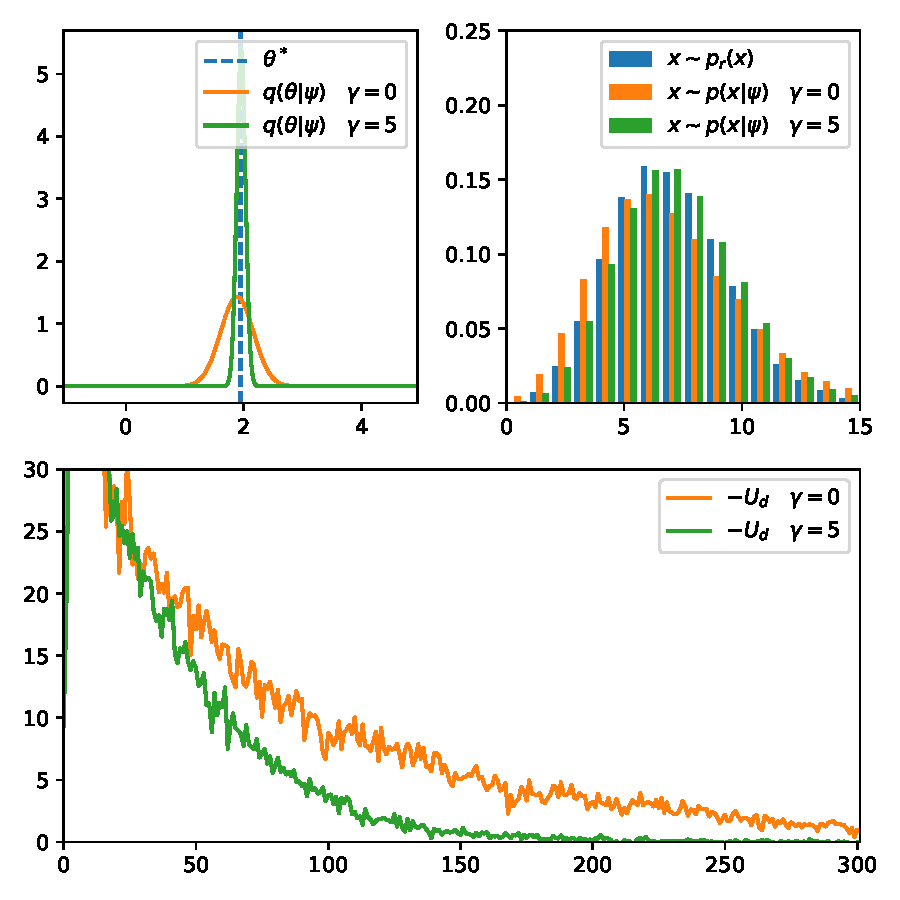
\includegraphics[width=0.48\textwidth]{figures/poisson.pdf}
    \caption{Discrete Poisson model with unknown mean.
             ({\it Top left}) Proposal distributions $q(\bftheta|\bfpsi)$ after adversarial variational optimization. For both $\gamma=0$ and $\gamma=5$, the distributions correctly concentrate their density around
                        the true value $\log(\lambda^*)$. Penalizing the entropy of the proposal distribution ($\gamma=5$) results in a tighter density.
             ({\it Top right}) Model distributions $\qxpsi$ after training. This plot shows that the resulting parameterizations of the simulator closely reproduce the true distribution.
             ({\it Bottom}) Empirical estimates of the variational upper bound $U_d$ as optimization progresses.
             }\label{fig:poisson}
\end{figure}

The top left plot in Figure~\ref{fig:poisson} illustrates the resulting proposal
distributions $q(\bftheta|\bfpsi)$ after AVO.  For
both $\gamma=0$ and $\gamma=5$, the proposal distributions correctly concentrate
their density around the true parameter value $\log(\lambda^*) = 1.94$. Under
the effect of the positive entropy penalty $H(q(\bftheta|\bfpsi))$,
the proposal distribution for $\gamma=5$ concentrates its mass more tightly,
yielding in this case a more precise inference.  The top right plot compares the
model distributions to the true distribution.  As theoretically expected from
adversarial training, we see that the resulting distributions closely match
the true distribution, with in this case visually slightly better results for the penalized
model.  The bottom plot of Figure~\ref{fig:poisson} shows empirical estimates
of $-U_d$ with respect to the epoch number. For both $\gamma=0$ and $\gamma=5$,
the curves quickly fall towards $0$, which indicates that
$\mathbb{E}_{\tilde{\mathbf{x}} \sim p(\mathbf{x}|\bftheta)}
[d(\tilde{\mathbf{x}};\bfphi)] \approx \mathbb{E}_{\mathbf{x} \sim
p_r(\mathbf{x})} [d(\mathbf{x};\bfphi)]$ and that the critic cannot distinguish
between true and model data. This confirms that adversarial variational optimization
works despite the discreteness of the data and lack of access to the
density $p(\bfx | \bftheta)$ or its gradient.

\subsection{Multidimensional continuous data}

As a second toy example, we consider a generator producing
5-dimensional continuous data, as originally specified in Section 4.2. of
\citep{cranmer2015approximating}. More specifically, we consider the following
generative process:
\begin{itemize}
    \item $\bfz = (z_0, z_1, z_2, z_3, z_4)$, such that \\
        $z_0 \sim {\cal N}(\mu=\alpha, \sigma=1)$,
        $z_1 \sim {\cal N}(\mu=\beta, \sigma=3)$,
        $z_2 \sim {\text{Mixture}}[\frac{1}{2}\,{\cal N}(\mu=-2, \sigma=1), \\  \frac{1}{2}\,{\cal N}(\mu=2, \sigma=0.5)]$,
        $z_3 \sim {\text{Exponential}(\lambda=3)}$, and
        $z_4 \sim {\text{Exponential}(\lambda=0.5)}$;
    \item $\mathbf{x} = R  \bfz$, where $R$ is a fixed
    semi-positive definite $5 \times 5$ matrix defining a fixed projection
    of $\bfz$ into the observed space.
\end{itemize}
Again, the AVO algorithm does not have access to the density or its gradient, only samples from the generative model
We consider observed data generated at the nominal values $\bftheta^* = (\alpha^*=1,\beta^*=-1)$.
The simulator parameters are modeled with a factored  (mean field) Gaussian
variational distribution $q(\bftheta|\bfpsi) = q(\alpha|\bfpsi) q(\beta|\bfpsi)$, where each component was
initialized with zero mean and unit variance.
Hyper-parameters are set to $M=64$, $n_\text{critic}=100$, $\lambda=0.025$, $\gamma=10$ and
Adam configured with $\alpha=0.01$, $\beta_1=0.9$ and $\beta_2=0.999$.
The network architecture of the critic is the same as in the previous example.


Starting with a proposal distribution $q(\bftheta|\bfpsi)$ largely spread over
the parameter space, as illustrated in the left plot of Figure~\ref{fig:multi},
AVO quickly converges towards a variational distribution whose density
concentrates around the nominal values $\bftheta^*$, as shown in the right plot of Figure~\ref{fig:multi}.
Overall, this example further illustrates and confirms the ability of adversarial
variational optimization for inference with multiple parameters and multidimensional
data, where reliable approximations of $p(\mathbf{x}|\bftheta)$ in a traditional
MLE setting would otherwise be difficult to construct.

\begin{figure}
    \centering
    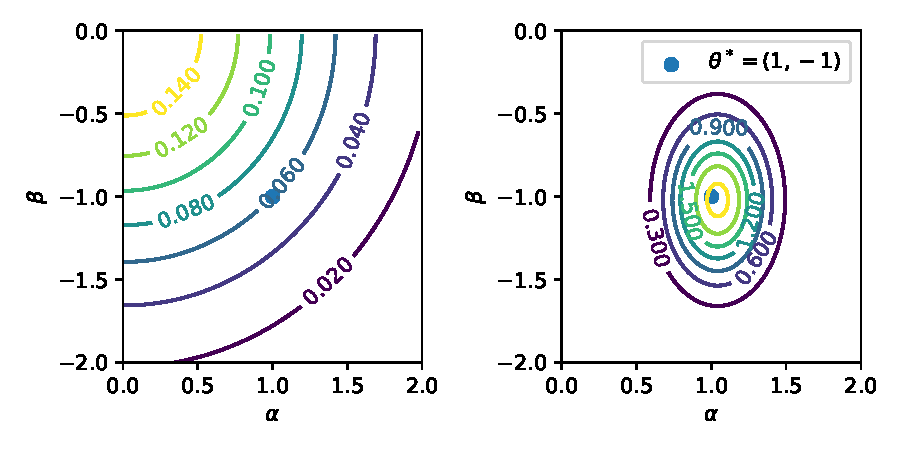
\includegraphics[width=0.48\textwidth]{figures/multi.pdf}
    \caption{Multidimensional continuous data.
             ({\it Left}) Density $q(\bftheta|\bfpsi)$ at the beginning of the procedure, for a proposal distribution initialized with zero mean and unit variance.
             ({\it Right}) Density $q(\bftheta|\bfpsi)$ after adversarial variational optimization ($\gamma=10$). The proposal density correctly converges towards a distribution whose density concentrates around $\bftheta^* = (1, -1)$.
             }\label{fig:multi}
\end{figure}


\subsection{Electron--positron annihilation}

\begin{figure}
    \centering
    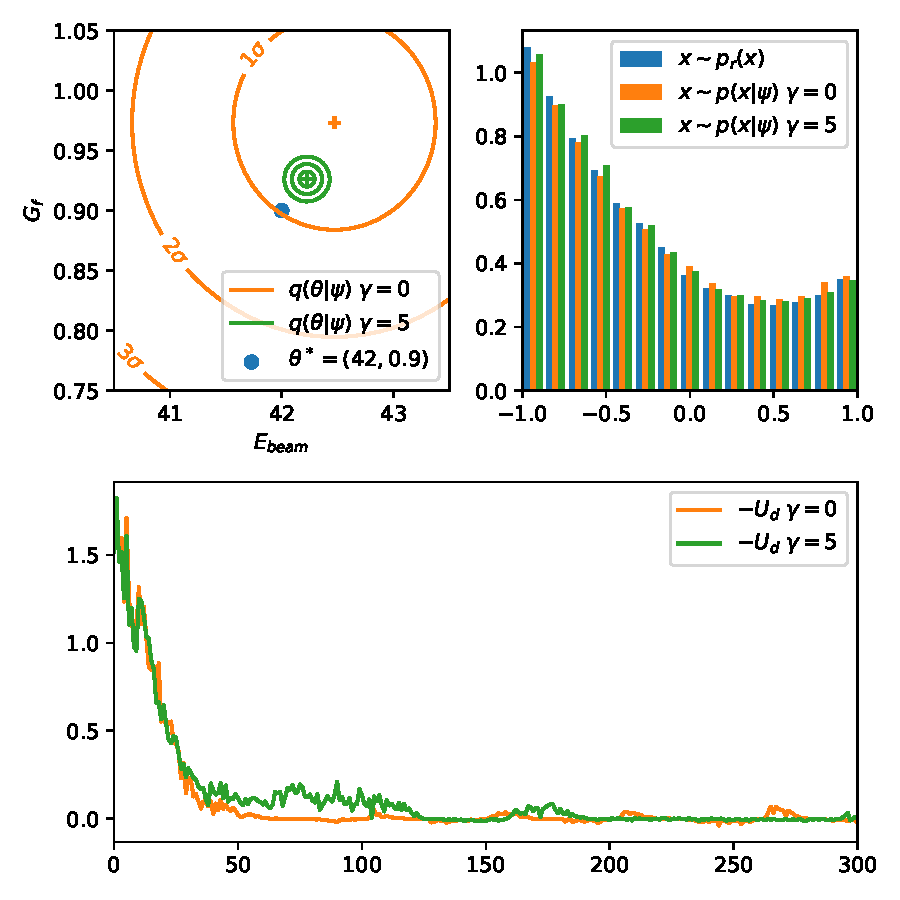
\includegraphics[width=0.48\textwidth]{figures/weinberg.pdf}
    \caption{Electron--positron annihilation.
    ({\it Top left}) Proposal distributions $q(\bftheta|\bfpsi)$ after adversarial variational optimization. The density of the penalized distribution ($\gamma=5$) is here highly concentrated, resulting in the green mass near $\bftheta^*$.
    ({\it Top right}) Model distributions $\qxpsi$ after training. Despite the differences between their respective proposal distributions, both models closely match the observed data.
    ({\it Bottom}) Empirical estimates of the variational upper bound $U_d$ as optimization progresses.
             }\label{fig:weinberg}
\end{figure}

As a more realistic example, we now consider a (simplified) simulator from
particle physics for electron--positron collisions resulting in muon--antimuon
pairs ($e^+e^- \rightarrow \mu^+\mu^-$). The simulator approximates the
distribution of observed measurements $\mathbf{x} = \cos(A) \in [-1,1]$, where $A$ is the
polar angle of the outgoing muon with respect  to the originally incoming
electron. Neglecting measurement uncertainty induced from the particle detectors,
this random variable is approximately distributed as
\begin{equation}\label{eq:simple_weinberg}
    p(\mathbf{x}|E_\text{beam}, G_f) = \frac{1}{Z} \left[ (1 + \mathbf{x}^2) + c(E_\text{beam}, G_f) \mathbf{x} \right]
\end{equation}
where $Z$ is a known normalization constant and $c$ is an asymmetry coefficient
function. Due to the linear term in the expression, the density $p(\mathbf{x} |
E_\text{beam}, G_f)$ exhibits a so-called {\it forward-backward} asymmetry.  Its
size depends on the values of the parameters $E_\text{beam}$ (the beam energy)
and $G_f$ (the Fermi constant) through the coefficient function $c$.

A typical physics simulator for this process includes a more precise treatment of the
quantum mechanical  $e^+e^- \rightarrow \mu^+\mu^-$ scattering
using \texttt{MadGraph}~\citep{Alwall:2011uj},  ionization of matter in the
detector due to the passage of the out-going $\mu^+\mu^-$ particles using
\texttt{GEANT4}~\citep{Agostinelli:2002hh}, electronic noise and other details of the sensors
that measure the ionization signal, and the deterministic algorithms that
estimate the polar angle $A$ based on the sensor readouts. The simulation of
this process is highly non-trivial as is the space of latent variables $\mathcal{Z}$.


%Given the
%known analytic form of the probability density function, a simulator for
%$\mathbf{x}$ can be implemented with rejection sampling~\citep{von195113}. As an
%arbitrary number of random drawings may be required before passing the
%acceptance threshold, this illustrates how the latent variable
%$\bfz$ does not necessarily need to be fixed-sized vector, and how its
%density  $p(\bfz|\bftheta)$ may depend on $\bftheta$ in some complicated way
%(Section~\ref{sec:problem}).

In this example, we consider observed data generated with the simplified generator of Eqn.~\ref{eq:simple_weinberg}
using $\bftheta^* = (E_\text{beam}^*=42, G_f^*=0.9)$. The simulator parameters are modeled with a
factored (mean field) Gaussian variational distribution $q(\bftheta|\bfpsi) = q(E_\text{beam}|\bfpsi)
q(G_f|\bfpsi)$, where each component is respectively initialized with mean $45$
and $1$ and variance $1$ and $0.01$. Hyper-parameters are set to $M=64$,
$n_\text{critic}=100$, $\lambda=0.0025$ and Adam configured with $\alpha=0.01$,
$\beta_1=0.9$ and $\beta_2=0.999$. As with the first example, we compare
entropy penalties $\gamma=0$ and $\gamma=5$.

The top left plot in Figure~\ref{fig:weinberg} illustrates the resulting
proposal distributions $q(\bftheta|\bfpsi)$ for $\gamma=0$ and $\gamma=5$ after
AVO. We see that the distributions both arrive
in the neighborhood of $\bftheta^*$, with a density  more highly concentrated for
$\gamma=5$ than for $\gamma=0$.  Despite these differences and the relative
distance with $\bftheta^*$, both models closely match the observed data, as shown
in the top right plot of  Figure~\ref{fig:weinberg}, with again slightly better
results for the entropy penalized model. This suggests either a relatively flat
landscape around $\bftheta^*$ or that the observed data can in this case also be
reproduced with the posterior predictive distribution $\qxpsi$.
Finally, the bottom plot of Figure~\ref{fig:weinberg} shows that for both
$\gamma=0$ and $\gamma=5$ the variational upper bound $-U_d$ quickly fall
towards $0$, which indicates  convergence towards a distribution that the critic
cannot distinguish from the true distribution.
%In summary, despite the intricate
%relation between the observations $\mathbf{x}$, the latent variable $\bfz$
%and the parameters $\bftheta$, this example demonstrates the efficacy
%of AVO for parameter inference on a black box
%simulator.


% ==============================================================================

\section{Related work}

This work sits at the intersection of several lines of research related to
likelihood-free inference, approximate Bayesian computation (ABC),
implicit generative networks, and variational inference.
%Our focus
%is on extending existing work to non-differentiable generative models
%that do not admit a tractable density.
Viewed from the literature around implicit generative models based on neural networks,
the proposed method can be considered as a direct adaptation of
generative adversarial networks~\citep{goodfellow2014generative,2017arXiv170104862A, 2017arXiv170107875A} to
non-differentiable simulators using variational optimization~\cite{2012arXiv1212.4507S,staines2013optimization}.

Adversarial Learned Inference (ALI)~\citep{dumoulin2016adversarially},
Bidirectional GANs (BiGANs)~\citep{donahue2016adversarial},
$\alpha$-GAN~\citep{rosca2017variational}, Adversarial Variational Bayes
(AVB)~\citep{DBLP:journals/corr/MeschederNG17}, and the \texttt{PC-Adv}
algorithm of  \citep{2017arXiv170208235H}  are a recent extension to GANs that
add an inference network to the generative model.  Each of these assume a
tractable density $p(\bfx|\bftheta)$ that is differentiable with respect to
$\bftheta$, which is  not satisfied in the likelihood-free setting. Our lifting
of the non-differentiable simulator $p(\bfx|\bftheta)$ to the variational
program $q(\bfx | \bfpsi)$ provides the ability to differentiate expectations
with respect to $\bfpsi$ as in Eqn~\ref{eqn:approx-grad}; however, the density
$q(\bfx | \bfpsi)$ is still intractable. Moreover, we do not attempt to define a
recognition model $q(\bfz | \bftheta, \bfx)$ as the latent space $\mathcal{Z}$
of many real-world simulators is complicated and not amenable to neural a
recognition model.
%One similarity of our work to AVB is that the ELBO is rewritten such that the intractable term $\log p(\bfz) - \log q_\bfphi(\bfz | \bfx)$ is replaced with an optimized neural network $T(x,z)$, which structurally similar to the role of the critic $d$ in the Kantorovich-Rubinstein dual description of the WGAN.

%\kcnote{does \citep{rosca2017variational} go in the above paragraph?}

From the point of view of likelihood-free inference, where  non-differentiable
simulators are the norm, our contributions are threefold. First is the process
of lifting expectations with respect to the non-differentiable simulator
$\mathbb{E}_{\tilde{\bfx} \sim p(\bfx | \bftheta)}$ to a differentiable
expectations with respect to the variational program $\mathbb{E}_{\tilde{\bfx}
\sim q(\bfx | \bfpsi)}$. Secondly, is the introduction of a novel form of
variational inference that works in a likelihood-free setting. Thirdly, the
AVI-MC algorithm can be viewed as a form of empirical Bayes where the prior is
optimized based on the data.

%Fourthly, the AVL algorithm is not a Bayesian inference algorithm, but instead provides point estimates $\bftheta^*$.

Perhaps the closest to our work is~\cite{bernton2017inference}, which uses
Wasserstein distance both to find point estimates $\bftheta^*$ and as a part of
a rejection sampler in an ABC-like setup (as opposed to variational inference).
They emphasize that this approach allows one to eliminate the summary statistics
typically used in ABC and calculate the Wasserstein distance explicitly, without
making use of the Kantorovich-Rubinstein duality and of a critic $d$. For high-dimensional
data, they note that this is computationally expensive and introduce an
approximation based on projection of the data onto Hilbert space-filling curves.
Their Remark 5.1 points out that~\citep{montavon2016wasserstein} proposed an
approximation of the gradient of an entropy-regularized Wasserstein distance,
which uses a similar duality. They note that ``Unfortunately, it is not
applicable in the setting of purely generative models, as it involves point-wise
evaluations of the derivative of the log-likelihood.'' Thus, our contribution is
to provide gradients of an approximate MWE by taking expectations with the
variational program $q(\bfx | \bfpsi)$. This paired with the critic
Kantorovich-Rubinstein dual formulation of the Wasserstein distance
allows us to work in high dimensions without summary statistics and
optimize $\bfpsi$ with stochastic gradient descent. Additionally,
our our AVO-EB procedure avoids the inefficiencies of
their Wasserstein rejection sampler incurred from using the ABC-likelihood.

%\kcnote{We don't use ABC-likelihood (more efficient?) used here and in VBIL. We also don't specify a prior b/c it's like implicit empirical bayes. They also don't specify a recognition model to latents. }


%\kcnote{Could we actually replace the optimization of the critic with a direct Wasserstein distance calculation in fewer dimensions. If the data is drawn from the variational program, it would still be differentiable with respect to $\bfpsi$. No, because it still requires $\nabla_\psi \log p(\bfx | \bfpsi)$}



%Within the literature on ABC and likelihood-free inference,
%the closest to our work are procedures that rely on a classifier to estimate the
%discrepancy between the observed data and the model distributions. For example,
%\citep{gutmann2012noise} uses non linear logistic regression for fitting
%unnormalized differentiable statistical models. Similarly, \citep{cranmer2015approximating,cranmer2016experiments,2016arXiv161110242D} estimate likelihood
%ratios through supervised classification, which can in turn be used for
% Bayesian or frequentist inference. Similarly, \citep{gutmann2017likelihood}
% makes use of classification accuracy as
%a summary statistics for approximate Bayesian computation.



As reviewed in \cite{2016arXiv161003483M}, likelihood-free inference is
intimately tied to a class of algorithms that can be framed as density
estimation-by-comparison. In most cases, these inference algorithms are
formulated as an iterative two-step process where the model distribution is
first compared to the true data distribution and then updated to make it more
comparable to the latter. Relevant work in this direction includes
\citep{gutmann2012noise,cranmer2015approximating,cranmer2016experiments,2016arXiv161110242D,gutmann2017likelihood,rosca2017variational}.


%%In this context, the proposed method can be considered as a direct adaptation of
%%generative adversarial networks~\citep{goodfellow2014generative} to
%%non-differentiable simulators.
%It also constitutes an approximate gradient
%descent alternative to likelihood-free inference based on bayesian optimization and approximated density
%ratios~\citep{cranmer2015approximating,cranmer2016experiments} or to classifier
%ABC~\citep{gutmann2017likelihood}.

%This work has many connections to work on variational inference, in which the goal is to optimize the recognition model $q(\bfz, \bftheta|\bfpsi)$ so that it is close to the true posterior $p(\bfz, \bftheta |x)$.
%This is slightly different from variational optimization (or variational learning), where the goal is to find $\bftheta^*$ such that $p(\bfx|\bftheta^*) \approx p_r(\bfx)$.  Typically in variational inference the model $p(\bfx|\bftheta)$ admits a density, so that the likelihood is known. Thus, assuming the prior also admits a density, it is tractable to evaluate the posterior is (up to a constant factor). In Adversarial Variational Bayes \citep{DBLP:journals/corr/MeschederNG17} and, equivalently, the \texttt{PC-Adv} algorithm of  \citep{2017arXiv170208235H}), the authors use an adversarial setup, but assume a known density $p(\bfx|\bftheta)$ that is differentiable with respect to $\bftheta$.


This work has also many connections to work on variational inference, in which the
goal is to optimize the recognition model $q(\bfz, \bftheta|\bfpsi)$ so that it
is close to the true posterior $p(\bfz, \bftheta |\mathbf{x})$. There have been efforts
to extend variational inference to intractable likelihoods; however, they
require restrictive assumptions.  In \citep{tran2017variational}, the authors
consider Variational Bayes with an Intractable Likelihood (VBIL). In that
approach ``the only requirement is that the intractable likelihood can be
estimated unbiasedly.'' In the case of simulators, they propose to use the
ABC-likelihood with an $\epsilon$ kernel. The ABC likelihood is only unbiased as
$\epsilon > 0$,   thus this method inherits the drawbacks of the ABC-likelihood
including the choice of summary statistics and the inefficiency in evaluating
the ABC likelihood for high-dimensional data and small $\epsilon$.

%\kcnote{do we keep JC-Adv  notes? Should say something about Hamiltonian ABC}
%In \citep{2017arXiv170208235H} the author defines implicit distributions to be ``probability models whose probability density function may be intractable, but there is a way to 1) sample from them exactly and/or calculate and approximate expectations under them, and 2) calculate or estimate gradients of such expectations with respect to model parameters.'' This notion of implicit model does not include most scientific simulators as 2) is not satisfied. Furthermore, the  \texttt{JC-Adv} and \texttt{JC-Den} algorithm defined there applies to implicit models, but, as the author points out, is aimed at variational inference and ``does not provide a direct way to learn model parameters $\bftheta$''.
%``Unfortunately, none of the algorithms presented here allow for fully variational learning
%of model parameters $\bftheta$ when $p_\bftheta(\bfx|\bfz)$ is implicit.''
%%JC-Adv doesn't let you optimize theta, theta is fixed and you get variational inference on z. Need a recognition model for latents

In \citep{meeds2015hamiltonian}, the authors introduce Hamiltonian ABC which
applies in the likelihood-free setting, and they estimate gradients with respect
to $\bftheta$ through finite differences from multiple forward passes of the
simulator with variance reduction strategies based on controlling the source of
randomness used for the latent variable $\bfz$.

%\kcnote{F.H. Implicit model is differentiable. Is what we are doing JC-Adv with our variational program}

%\subsection{Operator Variational Optimization}

%Lastly, we make a connection to Operator Variational Inference (OPVI)~\citep{2016arXiv161009033R},
%which is a generalization of variational inference formulated as the following optimization problem
%\begin{eqnarray}
%\bflambda^* = \inf_\bfpsi \sup_\bflambda \mathbb{E}_{ \bfz \sim q( \bfz | \bflambda)} [ (O^{p,q} f_\bfphi) ] \, .
%\end{eqnarray}
%In traditional VI with the KL distance, this corresponds to $(O^{p,q} f) = \log q(z) - \log p(z|x) \, \forall f \in \mathcal{F}$.
%AVO can be cast into a similar form with expectations over $\bfx$ instead of $\bfz$ and
%\begin{eqnarray} \label{eq:opvi_avo}
%\bfpsi^* &=& \inf_\bfpsi \sup_\bfphi\mathbb{E}_{\bfx\sim p_r(\bfx)}[d(\bfx)] - \mathbb{E}_{\bfx \sim q(\bfx|\bfpsi)}[d(\bfx)] \\
%\label{eq:opvi_avo2} &=&  \inf_\bfpsi \sup_\bfphi \mathbb{E}_{ \bfx \sim q( \bfx | \bfpsi)} [ (O^{p_r,p_\bfpsi} d_\bfphi) ] \;.
%\end{eqnarray}
%Rewriting Eqn.~\ref{eq:opvi_avo} as Eqn.~\ref{eq:opvi_avo2} is possible through importance sampling
%and reinforces the link to density ratio estimation as this corresponds to the operator
%\begin{equation}
%(O^{p,q} d) = \left( \frac{p_r(\bfx)}{q(\bfx|\bfpsi)}  -1 \right) d(\bfx) \, .
%\end{equation}

Lastly, we make a connection to Operator Variational Inference (OPVI)~\citep{2016arXiv161009033R},
which is a generalization of variational inference formulated as the following optimization problem
\begin{eqnarray}
\bflambda^* = \inf_\bflambda \sup_\bfphi \mathbb{E}_{ \bfz \sim q( \bfz | \bflambda)} [ (O^{p,q} f_\bfphi) ] \, .
\end{eqnarray}
In traditional VI with the KL distance, this corresponds to $(O^{p,q} f) = \log q(\bfz) - \log p(\bfz|\bfx) \, \forall f \in \mathcal{F}$.
AVO can be cast into a similar form with expectations over $\bfx$ instead of $\bfz$ and
\begin{eqnarray} \label{eq:opvi_avo}
\bfpsi^* &=& \inf_\bfpsi \sup_\bfphi \mathbb{E}_{ \bfx \sim q( \bfx | \bfpsi)} [ (O^{p_r,p_\bfpsi} d_\bfphi) ] \\\
\label{eq:opvi_avo2} &=&  \inf_\bfpsi \sup_\bfphi\mathbb{E}_{\bfx\sim p_r(\bfx)}[d(\bfx)] - \mathbb{E}_{\bfx \sim q(\bfx|\bfpsi)}[d(\bfx)] \, .
\end{eqnarray}
Rewriting Eqn.~\ref{eq:opvi_avo} as Eqn.~\ref{eq:opvi_avo2} is possible through importance sampling,
corresponding to an implicit form of the operator
\begin{equation}
(O^{p,q} d) = \left( \frac{p_r(\bfx)}{q(\bfx|\bfpsi)}  -1 \right) d(\bfx) \, ,
\end{equation}
which reinforces the link to density ratio estimation and inference with implicit models.



%
%%\begin{equation}
%%(O^{p,q} f) = \log q(z) - \log p(z|x) \, \forall f \in \mathcal{F}
%%\end{equation}
%
%
%%This is natural here, but not quite OPVI formalism:
%%\begin{equation}
%%\bfpsi^* = \inf_\bfpsi \sup_\bfphi \mathbb{E}_{ \bftheta \sim q(\bftheta | \bfpsi)} [ (O^{p,q} f_\bfphi) ]
%%\end{equation}
%%
%%\begin{equation}
%%(O^{p,q} f) = W(p,q) = \sup_f \mathbb{E}_{x\sim p}[f(x)] - \mathbb{E}_{x \sim q}[f(x)]
%%\end{equation}
%%The expectation should be $x \sim p(x|\bfpsi)$ and here $(O^{p,q} f)$ is a scalar and not a function of $x$
%
%To get into OPVI formalism
%
%\begin{eqnarray}
%\bfpsi^* &=& \inf_\bfpsi \sup_\bfphi\mathbb{E}_{x\sim p_r(x)}[f(x)] - \mathbb{E}_{x \sim p(x|\bfpsi)}[f(x)] \\
%&=&  \inf_\bfpsi \sup_\bfphi \mathbb{E}_{ x \sim p( x | \bfpsi)} [ (O^{p_r,p_\bfpsi} f_\bfphi) ]
%\end{eqnarray}
%with
%\begin{equation}
%(O^{p,q} f) = \left( \frac{p_r(x)}{p(x|\bfpsi)}  -1 \right) f(x)
%\end{equation}

%We can think of $p(\bfx|\bfpsi)$ as a \textit{variational program} as described in ~\citep{2016arXiv161009033R}, though more complicated than the a simple reparametrization of normally distributed noise $\epsilon$ through a differentiable function $R(\epsilon, \bfpsi)$. In our case, the variational program is a marginalized non-differentiable simulator simulator.  Nevertheless, it can generate samples for $x$, is differentiable with respect to $\bfphi$, and its density is be intractable.



% ==============================================================================

\section{Summary}

In this note, we develop likelihood-free inference algorithms for non-differentiable, implicit generative models.
The algorithms combine adversarial training  with variational optimization to
minimize variational upper bounds  on the otherwise non-differentiable
adversarial objectives.
The AVO-EB algorithm enables empirical Bayesian through variational inference in the likelihood free setting.
This approach does not incur the inefficiencies of an ABC-like rejection sampler. The AVO-MWE algorithm
provides point estimates for the generative model, which asymptotically correspond to the data generating parameter when the model is well-specified. Both algorithms work on continuous or discrete observed data.

Preliminary results on toy problems with discrete and continuous data validate the proposed method.
While the obtained results are encouraging, the complete validation of the
method remains to be carried out in real conditions on a full fledged scientific
simulator -- which we plan to achieve for a next version of this work.
In terms of method, several components need to be further investigated.
First, we need to better study the interplay between the entropy penalty and the adversarial objectives.
Second, we should better understand the dynamics of the optimization
procedure, in particular when combined with momentum-based optimizers like Adam.
Third, we need to consider whether less noisy estimates of the gradients
$\nabla_\bfpsi U_g$ can be computed.
%, in particular by exploiting the fact in the composition $d(g(\bfz;\bftheta); \bfpsi)$
%the derivatives of $d$ are known exactly.

%We note that the technique can be used either to fit a generative model to an observed data distribution
%or to fit a fast simulator to a slower, higher-fidelity simulator.

%\kcnote{could also use this to tune non-differentialble fast simulator to slower full simulator. Then fixed data size not an issue}

%\kcnote{proposal distribution $\to$ variational distribution}

% ==============================================================================

\section*{Acknowledgments}

We would like to thank Lukas Heinrich for helpful comments regarding
the electron--positron annihilation simulation.

GL and KL are both supported through NSF ACI-1450310, additionally KC is
supported through PHY-1505463 and PHY-1205376.


% ==============================================================================

%\bibliographystyle{hacm}
\bibliographystyle{hunsrt}
\bibliography{bibliography.bib}


\end{document}
